\documentclass{article}
\newif\ifshowsolutions
\showsolutionstrue
\usepackage{listings}
\usepackage{amsmath}
\usepackage{subfig}
\usepackage{amsthm}
\usepackage{amsmath}
\usepackage{amssymb}
\usepackage{graphicx}
\usepackage{mdwlist}
\usepackage{geometry}
\usepackage{titlesec}
\usepackage{palatino}
\usepackage{mathrsfs}
\usepackage{fancyhdr}
\usepackage{paralist}
\usepackage{todonotes}
\usepackage{tikz}
\usepackage{float} % Place figures where you ACTUALLY want it
\usepackage{comment} % A hack to toggle sections
\usepackage{ifthen}
\usepackage{mdframed}
\usepackage{verbatim}
\usepackage{listings}
\usepackage{bbm}
\usepackage{upquote} % Prevents backticks replacing single-quotes in verbatim
\usepackage[strings]{underscore}
\usepackage[colorlinks=true]{hyperref}
\usetikzlibrary{positioning,shapes,backgrounds}

\geometry{margin=1in}
\geometry{headheight=2in}
\geometry{top=2in}

\setlength{\marginparwidth}{2.15cm}
\setlength{\parindent}{0em}
\setlength{\parskip}{0.6\baselineskip}

\rhead{}
\lhead{}

% Spacing settings.
\titlespacing\section{0pt}{12pt plus 2pt minus 2pt}{0pt plus 2pt minus 2pt}
\titlespacing\subsection{0pt}{12pt plus 4pt minus 2pt}{0pt plus 2pt minus 2pt}
\titlespacing\subsubsection{0pt}{12pt plus 4pt minus 2pt}{0pt plus 2pt minus 2pt}
\renewcommand{\baselinestretch}{1.15}

% Shortcuts for commonly used operators.
\newcommand{\E}{\mathbb{E}}
\newcommand{\Var}{\operatorname{Var}}
\newcommand{\Cov}{\operatorname{Cov}}
\newcommand{\Bias}{\operatorname{Bias}}
\DeclareMathOperator{\argmin}{arg\,min}
\DeclareMathOperator{\argmax}{arg\,max}

% Do not number subsections and below.
\setcounter{secnumdepth}{1}

% Custom format subsection.
\titleformat*{\subsection}{\large\bfseries}

% Set up the problem environment.
\newcounter{problem}[section]
\newenvironment{problem}[1][]
  {\begingroup
    \setlength{\parskip}{0em}
    \refstepcounter{problem}\par\addvspace{1em}\textbf{Problem~\Alph{problem}\!
    \ifthenelse{\equal{#1}{}}{}{ [#1 points]}:}
  \endgroup}

% Set up the subproblem environment.
\newcounter{subproblem}[problem]
\newenvironment{subproblem}[1][]
  {\begingroup
    \setlength{\parskip}{0em}
    \refstepcounter{subproblem}\par\medskip\textbf{\roman{subproblem}.\!
    \ifthenelse{\equal{#1}{}}{}{ [#1 points]:}}
  \endgroup}

% Set up the teachers and materials commands.
\newcommand\teachers[1]
  {\begingroup
    \setlength{\parskip}{0em}
    \vspace{0.3em} \textit{\hspace*{2em} TAs responsible: #1} \par
  \endgroup}
\newcommand\materials[1]
  {\begingroup
    \setlength{\parskip}{0em}
    \textit{\hspace*{2em} Relevant materials: #1} \par \vspace{1em}
  \endgroup}

% Set up the hint environment.
\newenvironment{hint}[1][]
  {\begin{em}\textbf{Hint: }}
  {\end{em}}


% Set up the solution environment.
\ifshowsolutions
  \newenvironment{solution}[1][]
    {\par\medskip \begin{mdframed}\textbf{Solution~\Alph{problem}#1:} \begin{em}}
    {\end{em}\medskip\end{mdframed}\medskip}
  \newenvironment{subsolution}[1][]
    {\par\medskip \begin{mdframed}\textbf{Solution~\Alph{problem}#1.\roman{subproblem}:} \begin{em}}
    {\end{em}\medskip\end{mdframed}\medskip}
\else
  \excludecomment{solution}
  \excludecomment{subsolution}
\fi

\lstset{upquote=true}



%%%%%%%%%%%%%%%%%%%%%%%%%%%%%%
% HEADER
%%%%%%%%%%%%%%%%%%%%%%%%%%%%%%

\chead{
  {\vbox{
      \vspace{2mm}
      \large
      Machine Learning \& Data Mining \hfill
      Caltech CS/CNS/EE 155 \hfill \\[1pt]
      Set 3\hfill
      October $13^\text{th}$, 2026 \\
    }
  }
}

\begin{document}
\pagestyle{fancy}



%%%%%%%%%%%%%%%%%%%%%%%%%%%%%%
% POLICIES
%%%%%%%%%%%%%%%%%%%%%%%%%%%%%%

\section*{Policies}
\begin{itemize}
	\item Due 11:59 PM PT, October $20^\text{th}$, 2026, via Gradescope.
	\item You are free to collaborate on all of the problems, subject to the collaboration policy stated in the syllabus.
	\item In this course, we will be using Google Colab for code submissions. You will need a Google account.
	\item Homework will be graded on completion, but you must make a good-faith effort. No late submissions will be accepted.
	\item Students are expected to complete homework assignments based on their understanding of the course material. Student can use LLMs as a resource (e.g., helping with debugging, or grammar checking), but the assignments (including code) should be principally authored by the student.
\end{itemize}

\section*{Submission Instructions}
\begin{itemize}
	\item Submit your report as a single .pdf file to Gradescope (entry code PRGP5Z), under "Problem Set 3".
	\item In the report, \textbf{include any images generated by your code} along with your answers to the questions.
	\item Submit your code by \textbf{sharing a link in your report} to your Google Colab notebook for each problem (see naming instructions below). Make sure to set sharing permissions to at least "Anyone with the link can view".
	\item For instructions specifically pertaining to the Gradescope submission process, see \url{https://www.gradescope.com/get_started#student-submission}.
\end{itemize}

\section*{Google Colab Instructions}
For each notebook, you need to save a copy to your drive.
\begin{enumerate}
        \item Open the github preview of the notebook, and click the icon to open the colab preview.
        \item On the colab preview, go to File $\rightarrow$ Save a copy in Drive.
        \item Edit your file name to “lastname_firstname_set_problem”, e.g.”yue_yisong_set3_prob1.ipynb”
\end{enumerate}



%%%%%%%%%%%%%%%%%%%%%%%%%%%%%%
% PROBLEM 1
%%%%%%%%%%%%%%%%%%%%%%%%%%%%%%

\newpage
\section{Decision Trees [30 Points]}
\materials{Lecture 5}

\problem[7]
Consider the following data, where given information about some food you must predict whether it is healthy:

\begin{table}[ht]
\centering
\begin{tabular}{c | c c c | c}
\hline
No. & Package Type & Unit Price $>$ \$5 & Contains $>$ 5 grams of fat & Healthy? \\ [0.5ex]
\hline
1 & Canned & Yes & Yes & No  \\
2 & Bagged & Yes & No  & Yes \\
3 & Bagged & No  & Yes & Yes \\
4 & Canned & No  & No  & Yes \\ [1ex]
\hline
\end{tabular}
\end{table}

Train a decision tree by hand using top-down greedy induction. Use \emph{entropy} (with natural log) as the impurity measure.  Since the data can be classified
without error, the stopping criterion will be no impurity in the leaves.

Submit a drawing of your tree showing the impurity reduction yielded by each split (including root) in your decision tree.

\begin{solution}
\upshape
At the root, $H = -\tfrac14\ln\tfrac14-\tfrac34\ln\tfrac34 \approx 0.562$. Each of the three attributes sends one pure pair
to one side and a 50/50 pair to the other, so the weighted child entropy is $\tfrac12\ln 2\approx 0.347$ and every root split
reduces entropy by $0.562-0.347 = 0.216$. This is a three-way tie, so I split on Package Type.
The Bagged branch $\{2,3\}$ is already pure. The Canned branch $\{1,4\}$ has $H=\ln 2\approx 0.693$;
splitting on fat (price works equally well) gives two pure leaves, a reduction of $0.693$
(or $0.347$ counted over the whole dataset). The two reductions add up to $0.216+0.347=0.562=H_\text{root}$, so no impurity is left.

\begin{center}
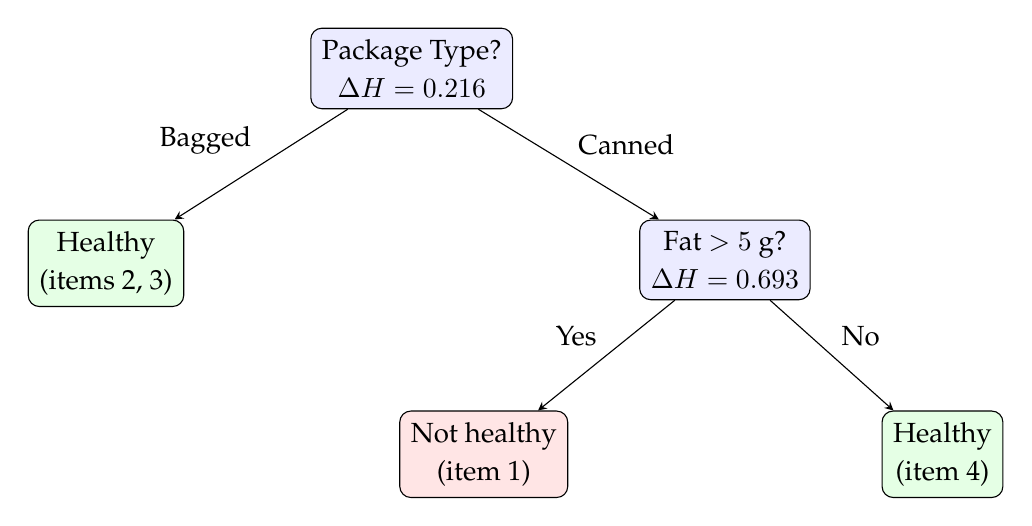
\begin{tikzpicture}[
  box/.style={draw, rounded corners, align=center, inner sep=4pt, fill=blue!8},
  leaf/.style={draw, rounded corners, align=center, inner sep=4pt, fill=green!10},
  bad/.style={draw, rounded corners, align=center, inner sep=4pt, fill=red!10},
  >=stealth]
  \node[box] (r) {Package Type?\\ $\Delta H = 0.216$};
  \node[leaf, below left=1.4cm and 1.6cm of r] (b) {Healthy\\ (items 2, 3)};
  \node[box, below right=1.4cm and 1.6cm of r] (c) {Fat $>5$ g?\\ $\Delta H = 0.693$};
  \node[bad, below left=1.4cm and 0.9cm of c] (u) {Not healthy\\ (item 1)};
  \node[leaf, below right=1.4cm and 0.9cm of c] (h) {Healthy\\ (item 4)};
  \draw[->] (r) -- node[above left] {Bagged} (b);
  \draw[->] (r) -- node[above right] {Canned} (c);
  \draw[->] (c) -- node[above left] {Yes} (u);
  \draw[->] (c) -- node[above right] {No} (h);
\end{tikzpicture}
\end{center}
\end{solution}

\problem[4]
Compared to a linear classifier, is a decision tree always preferred for classification problems? If not, draw a simple 2-D dataset that can be perfectly classified by a simple linear classifier but which requires an overly complex decision tree to perfectly classify.

\begin{solution}
\upshape
No. A tree can only make axis-aligned cuts, so when the true boundary is oblique it has to approximate it with a staircase.
In the figure, one line ($x_2=x_1$) separates all 16 points, while the tree needs 8 splits, and the number of splits
grows with the number of points. Such a tree is also hard to read and sensitive to small changes in the data, so it
overfits more easily than the linear model.

\begin{center}
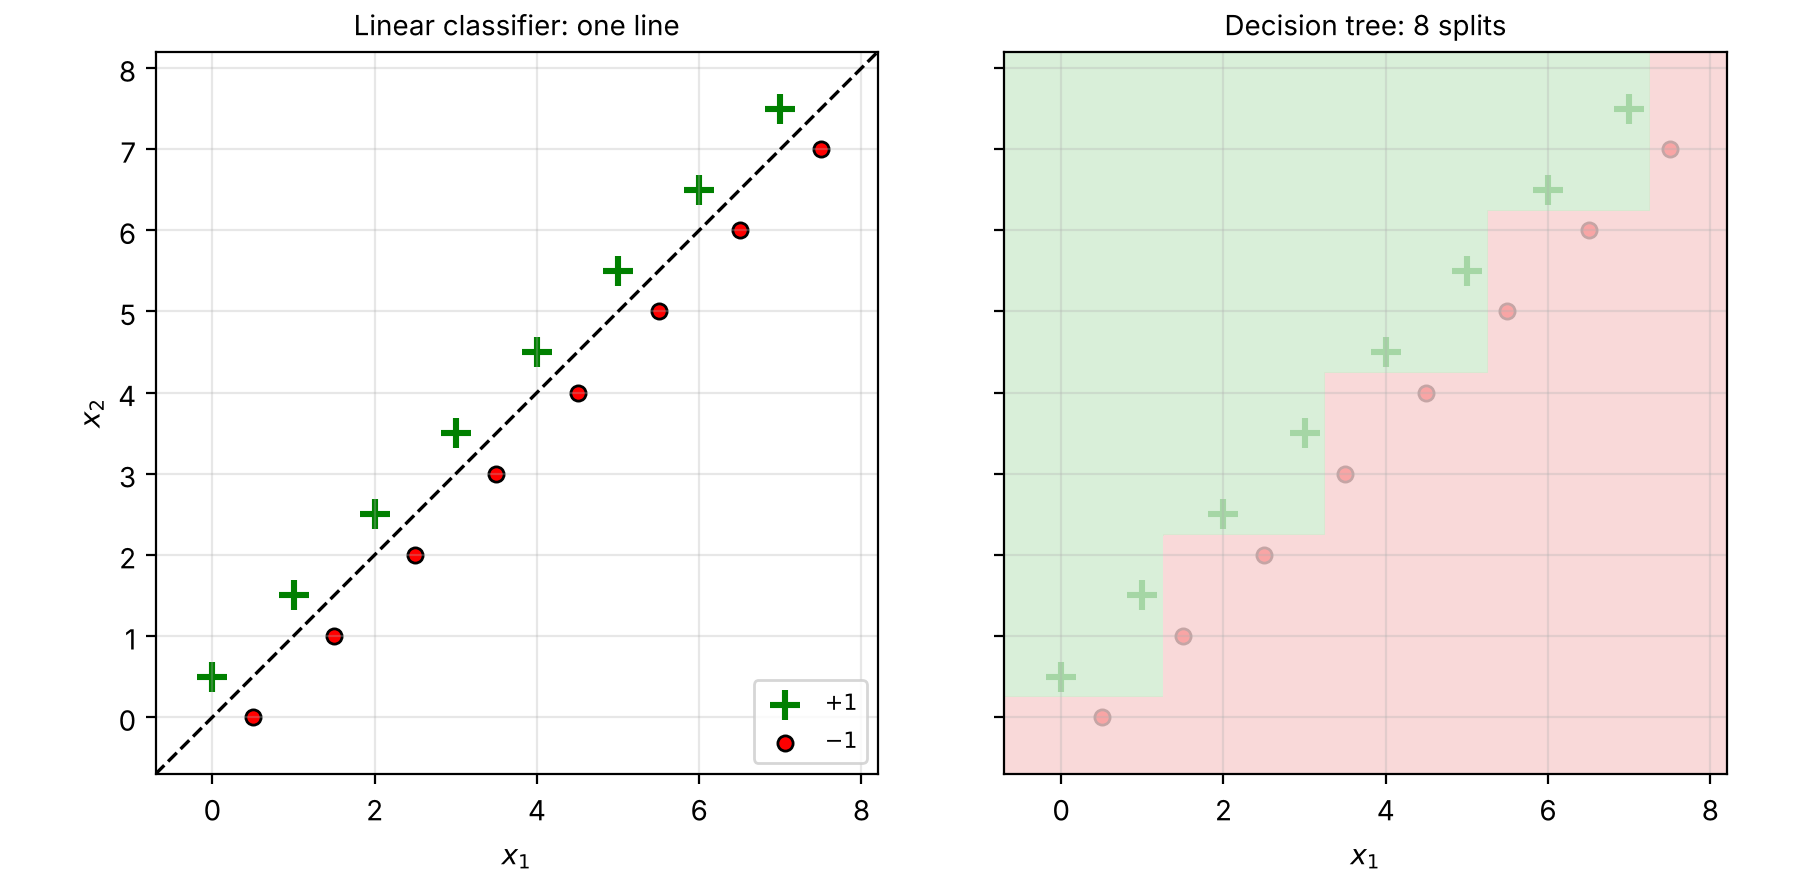
\includegraphics[width=0.85\textwidth]{../figs/prob1b_mine.png}
\end{center}
\end{solution}

\problem[15]
Consider the following 2D data set:
\begin{figure}[H]
    \begin{center}
    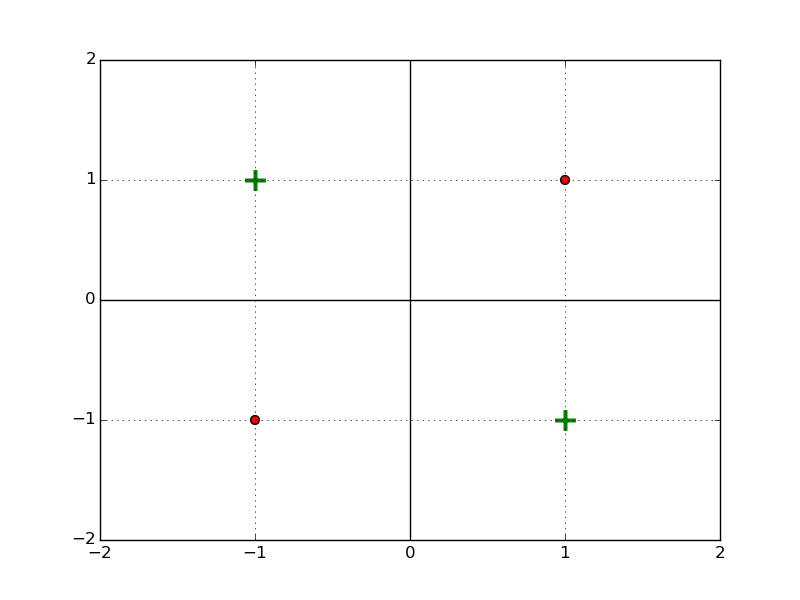
\includegraphics[width=3.3in]{../figs/1C_problem.png}
    \end{center}
    \end{figure}

\subproblem[5] Suppose we train a decision tree on this dataset using top-down greedy induction, with the Gini index as
the impurity measure. We define our stopping condition to be if no split of a node
results in any reduction in impurity. Submit a drawing of the resulting tree.  What is its classification error ((number of misclassified points) / (number of total points))?

\subproblem[5] Submit a drawing of a two-level decision tree that classifies the above dataset with zero classification error.  (You don't need to use any particular training algorithm to produce the tree.)

Is there any impurity measure (i.e. any function that maps the data points under a particular node in a tree to a real number) that would have led top-down greedy induction with the same stopping condition to produce the tree you drew?  If so, give an example of one, and briefly describe its pros and cons as an impurity measure for training decision trees in general (on arbitrary datasets). 

\subproblem[5] Suppose there are 100 data points in some 2-D dataset. What is the largest number of unique thresholds (i.e., internal nodes) you might need in order to achieve zero classification training error (on the training set)? Please
justify your answer.

\begin{solution}
\upshape
\textbf{i.} The root has Gini $1-(\tfrac12)^2-(\tfrac12)^2=\tfrac12$. Any threshold on $x_1$ or $x_2$ that splits the data
puts exactly one $+$ and one $\circ$ on each side, so both children also have Gini $\tfrac12$ and the weighted
impurity does not change. (Thresholds outside $[-1,1]$ leave one child empty.) No split reduces the impurity, so training stops at
the root: the tree is a single leaf, which predicts one class for every point. Its classification error is $2/4 = 50\%$.

\begin{center}
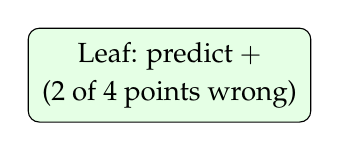
\begin{tikzpicture}[leaf/.style={draw, rounded corners, align=center, inner sep=5pt, fill=green!10}]
  \node[leaf] {Leaf: predict $+$\\ (2 of 4 points wrong)};
\end{tikzpicture}
\end{center}

\textbf{ii.} Split on $x_1>0$ at the root and on $x_2>0$ in both children; all four points are classified correctly.

\begin{center}
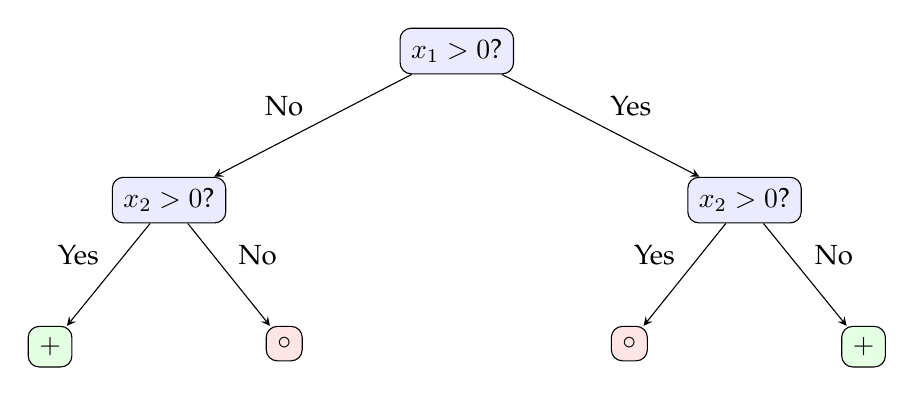
\begin{tikzpicture}[
  box/.style={draw, rounded corners, align=center, inner sep=4pt, fill=blue!8},
  leaf/.style={draw, rounded corners, align=center, inner sep=4pt, fill=green!10},
  bad/.style={draw, rounded corners, align=center, inner sep=4pt, fill=red!10},
  >=stealth]
  \node[box] (r) {$x_1>0$?};
  \node[box, below left=1.3cm and 2.2cm of r] (l) {$x_2>0$?};
  \node[box, below right=1.3cm and 2.2cm of r] (q) {$x_2>0$?};
  \node[leaf, below left=1.3cm and 0.5cm of l] (l1) {$+$};
  \node[bad, below right=1.3cm and 0.5cm of l] (l2) {$\circ$};
  \node[bad, below left=1.3cm and 0.5cm of q] (q1) {$\circ$};
  \node[leaf, below right=1.3cm and 0.5cm of q] (q2) {$+$};
  \draw[->] (r) -- node[above left] {No} (l);
  \draw[->] (r) -- node[above right] {Yes} (q);
  \draw[->] (l) -- node[above left] {Yes} (l1);
  \draw[->] (l) -- node[above right] {No} (l2);
  \draw[->] (q) -- node[above left] {Yes} (q1);
  \draw[->] (q) -- node[above right] {No} (q2);
\end{tikzpicture}
\end{center}

Entropy, Gini and misclassification error are all functions of the class proportions in the children. Here the first split leaves
every child at 50/50, so none of them can see any progress. A measure that works must look beyond the current proportions.
Example: $I(S)=$ the lowest classification error that any single split (stump) can reach on $S$.
Then $I(\text{root})=\tfrac12$ (every stump makes 2 errors out of 4), while after splitting on $x_1$ each child can be split perfectly on $x_2$, so $I=0$ for both.
The reduction is positive, greedy induction takes this split, and the children are pure, giving exactly the tree above.

\emph{Pros:} it detects feature interactions such as XOR that one-step impurity measures miss.
\emph{Cons:} every candidate split now needs its own search over stumps, which multiplies the training cost by roughly $ND$; it still
looks only one step ahead (parity of three features would fool it); and, being based on 0/1 error, it is flat in many situations, like the misclassification rate.

\textbf{iii.} The answer is $99$. \emph{Upper bound:} assume no two identical points have different labels (otherwise zero error is impossible). Any node with at least two distinct points can be split
by a threshold on a coordinate where they differ, so we can keep splitting until every leaf holds a single point. That gives at most $100$ leaves, and a binary tree with $L$ leaves has $L-1$ internal nodes, so at most $99$ thresholds.
\emph{This is attained:} put the points at $(k,k)$, $k=1,\dots,100$, with alternating labels. A leaf is an axis-aligned box, and a box containing $(a,a)$ and $(b,b)$ also contains every $(k,k)$ between them, hence two neighbours with different labels.
So every leaf may hold at most one point, which requires $100$ leaves and $99$ thresholds.
\end{solution}

\problem[4] Suppose in top-down greedy induction we want to split a leaf node that contains N data points composed of
D continuous features. What is the worst-case
complexity (big-O in terms of N and D) of the number of possible splits we must consider in order to find the one that most reduces impurity? Please justify your answer.

Note: Recall that at each node-splitting step in training a DT, you must consider all possible splits that you can make. While there are an infinite number of possible decision boundaries since we are using continuous features, there are not an infinite number of boundaries that result in unique child sets (which is what we mean by ``split'').



\begin{solution}
\upshape
$O(ND)$. For one continuous feature, sort the $N$ values. Two thresholds give the same split whenever they fall between the same pair of consecutive values, so there are at most $N-1$ distinct splits per feature.
Over $D$ features that is at most $D(N-1)=O(ND)$ splits. (If we sort once per feature and update the class counts as the threshold sweeps, each split is scored in $O(1)$, so finding the best one costs $O(DN\log N)$ in total.)
\end{solution}




\newpage


\section{Overfitting Decision Trees [30 Points]}
\materials{Lecture 5}

In this problem, you will use the Diabetic Retinopathy Debrecen Data Set, which contains features extracted from images to determine whether or not the images contain signs of diabetic retinopathy. Additional information about this dataset can be found at the link below:

\url{https://archive.ics.uci.edu/ml/datasets/Diabetic+Retinopathy+Debrecen+Data+Set}

In the following question, your goal is to predict the diagnosis of diabetic retinopathy, which is the final column in the data matrix.  Use the first 900 rows as training data, and the last
251 rows as validation data. Please feel free to use additional packages such as Scikit-Learn. Include your code in your submission.

\indent\problem[7] % indent for consistency
Train a decision tree classifier using Gini as the impurity measure and minimal leaf node size as early stopping criterion. Try different minimal leaf node sizes from 1 to 25 in increments of 1. Then, on a single plot, plot both training and test classification error versus leaf node size. To do this, fill in the \texttt{classification_err} and \texttt{eval_tree_based_model_min_samples} functions in the code template for this problem.

\begin{solution}
\upshape
Code (the notebook is based on the provided template): \url{https://colab.research.google.com/drive/PASTE_YOUR_PROB2_LINK}

\begin{lstlisting}[language=Python, basicstyle=\ttfamily\footnotesize, breaklines=true, frame=single]
def classification_err(y, real_y):
    err = np.mean(np.asarray(y) != np.asarray(real_y))
    return float(err)

def eval_tree_based_model_min_samples(clf, min_samples_leaf, X_train, y_train, X_test, y_test):
    train_err, test_err = [], []
    for m in min_samples_leaf:
        clf.set_params(min_samples_leaf=int(m))
        clf.fit(X_train, y_train)
        train_err.append(classification_err(clf.predict(X_train), y_train))
        test_err.append(classification_err(clf.predict(X_test), y_test))
    return np.array(train_err), np.array(test_err)
\end{lstlisting}

\begin{center}
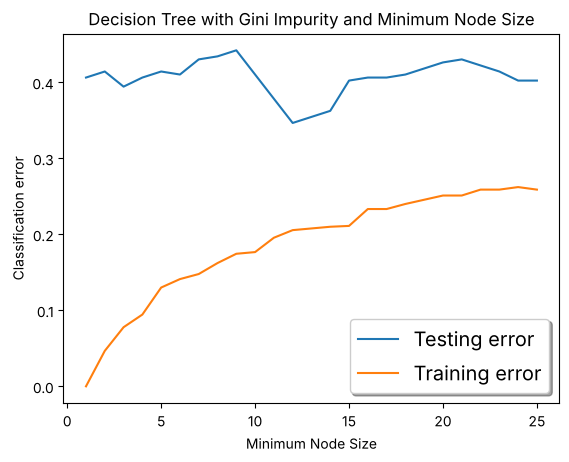
\includegraphics[width=0.55\textwidth]{../figs/fig2a.png}
\end{center}
\end{solution}

\problem[7]
Train a decision tree classifier using Gini as the impurity measure and maximal tree depth as early stopping criterion. Try different tree depths from 2 to 20 in increments of 1. Then, on a single plot, plot both training and test classification error versus tree depth. To do this, fill in the \texttt{eval_tree_based_model_max_depth} function in the code template for this problem.

\begin{solution}
\upshape
\begin{lstlisting}[language=Python, basicstyle=\ttfamily\footnotesize, breaklines=true, frame=single]
def eval_tree_based_model_max_depth(clf, max_depth, X_train, y_train, X_test, y_test):
    train_err, test_err = [], []
    for d in max_depth:
        clf.set_params(max_depth=int(d))
        clf.fit(X_train, y_train)
        train_err.append(classification_err(clf.predict(X_train), y_train))
        test_err.append(classification_err(clf.predict(X_test), y_test))
    return np.array(train_err), np.array(test_err)
\end{lstlisting}

\begin{center}
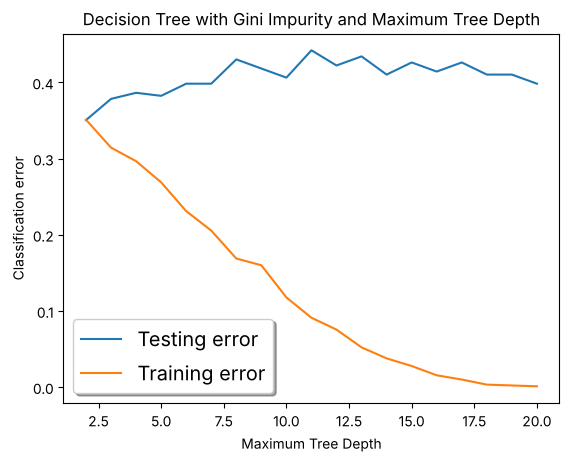
\includegraphics[width=0.55\textwidth]{../figs/fig2b.png}
\end{center}
\end{solution}

\problem[4]
For both the minimal leaf node size and maximum depth parameters tested in the last two questions, which parameter value minimizes the test error? What effects does early stopping have on the performance of a decision tree model?
Please justify your answer based on the two plots you derived.

\begin{solution}
\upshape
The test error is lowest at a minimum leaf size of \textbf{12} (test error $0.347$) and at a maximum depth of \textbf{2} (test error $0.351$).

Early stopping limits how closely the tree can fit the training set. Training error rises as the constraint gets tighter
(from $0$ at leaf size $1$ to about $0.26$ at $25$), and it falls to almost $0$ as depth grows to $20$.
Test error moves the other way: the almost fully grown trees (leaf size $1$: $0.406$; depth $20$: $0.398$) memorize the training set but generalize worse than the restricted ones ($0.347$ and $0.351$).
For depth, the test error mostly rises as the tree gets deeper, which is the classic overfitting pattern.
The leaf-size curve is noisier and only dips in the 10--14 range. Since the test set has just 251 points
(one point is $0.4\%$), I would trust the overall trend more than the exact argmin.
\end{solution}

\indent\problem[2] % indent for consistency
Train a random forest classifier using Gini as the impurity measure, minimal leaf node size as early stopping criterion, and 1,000 trees in the forest. Try different node sizes from 1 to 25 in increments of 1. Then, on a single plot, plot both training and test classification error versus
leaf node size.

\begin{solution}
\upshape
\begin{center}
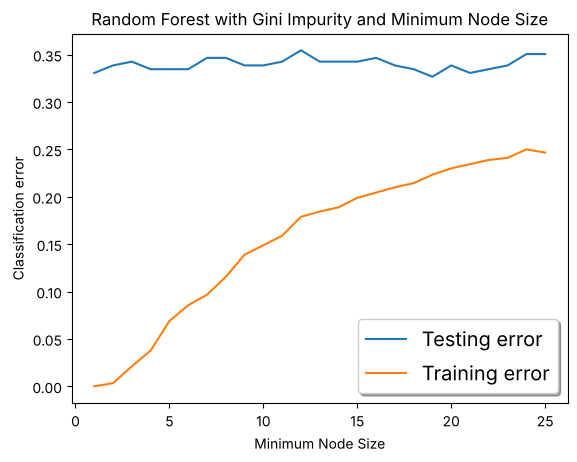
\includegraphics[width=0.55\textwidth]{../figs/fig2d.png}
\end{center}
\end{solution}

\problem[2]
Train a random forest classifier using Gini as the impurity measure, maximal tree depth as early stopping criterion, and 1,000 trees in the forest. Try different tree depths from 2 to 20 in increments of 1. Then, on a single plot, plot both training and test classification error versus tree depth.

\begin{solution}
\upshape
\begin{center}
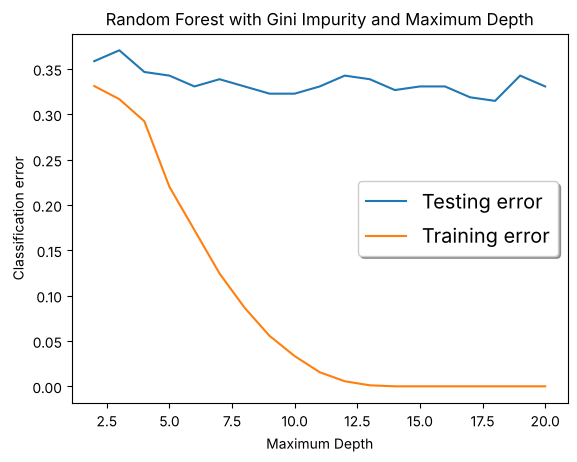
\includegraphics[width=0.55\textwidth]{../figs/fig2e.png}
\end{center}
\end{solution}

\problem[4]
For both the minimal leaf node size and maximum depth parameters tested, which parameter value minimizes the random forest test error? What effects does early stopping have on the performance of a random forest model?
Please justify your answer based on the two plots you derived.

\begin{solution}
\upshape
The random forest's test error is lowest at a minimum leaf size of \textbf{19} ($0.327$) and a maximum depth of \textbf{18} ($0.315$).
Both curves are very flat, though: the test error stays between about $0.31$ and $0.37$ for every setting, and the best and typical values differ by only a few of the 251 test points.

So early stopping has little effect on a random forest. The training error behaves as for a single tree (it reaches $0$ for leaf size 1 and for depth $\ge 13$),
but the test error does not get worse when the trees are grown fully; if anything, deeper trees are slightly better
(depth 2: $0.359$ vs.\ depth 18: $0.315$). Unlike a single tree, a forest does not need early stopping to avoid overfitting.
\end{solution}

\problem[4]
Do you observe any differences between the curves for the random forest and decision tree plots? If so, explain what could account for these differences.

\begin{solution}
\upshape
Yes. (1) The forest's test error is lower than the single tree's ($\approx 0.31$--$0.35$ vs.\ $0.35$--$0.44$) and its curves are much flatter and smoother. A single tree's test error goes up as it gets more complex and jumps around from one setting to the next.
(2) The reason is variance. A fully grown tree has low bias but high variance: a small change in the training set gives a different tree.
A random forest averages 1000 trees trained on bootstrap samples with random feature subsets, so their individual errors are partly decorrelated and the average has much lower variance
at about the same bias. This is why making the trees more complex hurts a single tree but not the forest, and why the forest does not need early stopping.
\end{solution}



\newpage
\section{The AdaBoost Algorithm [40 points]}
\materials{Lecture 6}

In this problem, you will show that the choice of the $\alpha_t$ parameter in
the AdaBoost algorithm corresponds to greedily minimizing an exponential upper
bound on the loss term at each iteration.

\problem[3]
Let $h_t: \mathbb{R}^m \rightarrow \{-1,1\}$ be the weak classifier obtained at step $t$, and let $\alpha_t$ be
its weight. Recall that the final classifier is $$H(x) = \text{sign}(f(x)) = \text{sign} \left(\sum\limits_{i=1}^T \alpha_{t}h_t(x) \right).$$

Suppose $\{(x_1, y_1), ..., (x_N, y_N)\} \subset \mathbb{R}^m \times \{-1,1\}$ is our training dataset.  Show that the training set error of the final classifier can be bounded from
above if an an exponential loss function is used:

$$E = \frac{1}{N} \sum\limits_{i=1}^N \exp(-y_{i}f(x_i)) \geq \frac{1}{N} \sum\limits_{i=1}^N \mathbbm{1}(H(x_i) \neq y_i),$$

where $\mathbbm{1}$ is the indicator function.

\begin{solution}
\upshape
Fix $i$. If $H(x_i)=y_i$, the indicator is $0$ and $\exp(-y_if(x_i))>0$. If $H(x_i)\neq y_i$, then $\operatorname{sign}(f(x_i))\ne y_i$, so $y_if(x_i)\le 0$ and $\exp(-y_if(x_i))\ge 1=\mathbbm 1(H(x_i)\neq y_i)$.
Either way $\exp(-y_if(x_i))\ge \mathbbm 1(H(x_i)\ne y_i)$. Averaging over $i=1,\dots,N$ gives $E\ge \frac1N\sum_i\mathbbm 1(H(x_i)\ne y_i)$.
\end{solution}

\problem[3]
Find $D_{T + 1}(i)$ in terms of $Z_t$, $\alpha_t$, $x_i$, $y_i$, and the classifier $h_t$, where $T$ is the last timestep and $t \in \{1, \ldots, T\}$. Recall that $Z_t$ is the normalization factor for distribution $D_{t+1}$:
$$Z_t = \sum\limits_{i=1}^N D_t(i) \exp(-\alpha_{t}y_{i}h_{t}(x_{i})).$$

\begin{solution}
\upshape
By definition $D_{t+1}(i)=\dfrac{D_t(i)\,e^{-\alpha_t y_ih_t(x_i)}}{Z_t}$ and $D_1(i)=\frac1N$. Unrolling the recursion,
\[
D_{T+1}(i)=\frac1N\prod_{t=1}^{T}\frac{e^{-\alpha_ty_ih_t(x_i)}}{Z_t}
=\frac{\exp\!\big(-y_i\sum_{t=1}^T\alpha_th_t(x_i)\big)}{N\prod_{t=1}^TZ_t}.
\]
\end{solution}

\problem[2]
Show that $E = \sum_{i=1}^N  \frac{1}{N} e^{\sum_{t=1}^T -\alpha_t y_i h_t(x_i)}.$

\begin{solution}
\upshape
Since $f(x_i)=\sum_{t=1}^T\alpha_th_t(x_i)$, we have $\exp(-y_if(x_i))=\exp\big(\sum_{t=1}^T-\alpha_ty_ih_t(x_i)\big)$. Substituting this into the definition of $E$ gives
$E=\sum_{i=1}^N\frac1N e^{\sum_{t=1}^T-\alpha_ty_ih_t(x_i)}$.
\end{solution}

\problem[5]
Show that
$$E = \prod\limits_{t=1}^T Z_t.$$

\begin{hint}
	Recall that $\sum_{i = 1}^N D_t(i) = 1$ because $D$ is a distribution.
\end{hint}

\begin{solution}
\upshape
$D_{T+1}$ is a distribution, so by Problem B and Problem C
\[
1=\sum_{i=1}^ND_{T+1}(i)=\frac{1}{\prod_{t=1}^TZ_t}\sum_{i=1}^N\frac1N e^{\sum_{t=1}^T-\alpha_ty_ih_t(x_i)}=\frac{E}{\prod_{t=1}^TZ_t}.
\]
Hence $E=\prod_{t=1}^TZ_t$.
\end{solution}

\problem[5]
Show that the normalizer $Z_t$ can be written as
\[Z_t = (1 - \epsilon_t) \exp(-\alpha_t) + \epsilon_{t} \exp(\alpha_t)\]
where $\epsilon_t$ is the training set error of weak classifier $h_t$ for the weighted dataset:
\[\epsilon_t = \sum\limits_{i=1}^N D_t(i)\mathbbm1(h_t(x_i) \neq y_i).\]

\begin{solution}
\upshape
Since $y_i,h_t(x_i)\in\{-1,1\}$, $y_ih_t(x_i)=1$ if $h_t$ classifies $x_i$ correctly and $-1$ otherwise. Split the sum in $Z_t$ accordingly:
\[
Z_t=\sum_{i:\,h_t(x_i)=y_i}D_t(i)e^{-\alpha_t}+\sum_{i:\,h_t(x_i)\ne y_i}D_t(i)e^{\alpha_t}
=(1-\epsilon_t)e^{-\alpha_t}+\epsilon_te^{\alpha_t},
\]
because the weight of the misclassified points is $\epsilon_t$ and, as $D_t$ sums to $1$, the weight of the correct ones is $1-\epsilon_t$.
\end{solution}

\problem[2]
We derived all of this because it is hard to directly minimize the training set error, but we can greedily minimize the upper bound $E$ on this error. Show that choosing $\alpha_t$
greedily to minimize $Z_t$ at each iteration leads to the choices in
AdaBoost:
$$\alpha_{t}^* = \frac{1}{2} \ln \left(\frac{1 - \epsilon_t}{\epsilon_t} \right).$$

\begin{solution}
\upshape
Assume $0<\epsilon_t<1$. Differentiating $Z_t(\alpha)=(1-\epsilon_t)e^{-\alpha}+\epsilon_te^{\alpha}$ gives $Z_t'(\alpha)=-(1-\epsilon_t)e^{-\alpha}+\epsilon_te^{\alpha}$. Setting this to $0$:
\[
e^{2\alpha}=\frac{1-\epsilon_t}{\epsilon_t}\quad\Longrightarrow\quad \alpha_t^*=\frac12\ln\frac{1-\epsilon_t}{\epsilon_t}.
\]
Since $Z_t''(\alpha)=Z_t(\alpha)>0$, $Z_t$ is convex and this stationary point is the global minimum.
\end{solution}

\begin{problem}[14]
    Implement the \texttt{GradientBoosting.fit()} and \texttt{AdaBoost.fit()} methods in the notebook provided for you. Some important notes and guidelines follow:
    \begin{itemize}
        \item For both methods, make sure to work with the class attributes provided to you. Namely, after \texttt{GradientBoosting.fit()} is called, \texttt{self.clfs} should be appropriately filled with the \texttt{self.n_clfs} trained weak hypotheses. Similarly, after \texttt{AdaBoost.fit()} is called, \texttt{self.clfs} and \texttt{self.coefs} should be appropriately filled with the \texttt{self.n_clfs} trained weak hypotheses and their coefficients, respectively.
        \item \texttt{AdaBoost.fit()} should additionally return an $(N, T)$ shaped numpy array \texttt{D} such that \texttt{D[:, t]} contains $D_{t+1}$ for each $t \in \{0, \ldots, \texttt{self.n_clfs}\}$.
        \item For the \texttt{AdaBoost.fit()} method, \textbf{use the 0/1 loss} instead of the exponential loss.
	\item The only Sklearn classes that you may use in implementing your boosting fit functions are the DecisionTreeRegressor and DecisionTreeClassifier, not GradientBoostingRegressor.
    \end{itemize}
\end{problem}

\begin{solution}
\upshape
Code (the notebook is based on the provided template): \url{https://colab.research.google.com/drive/PASTE_YOUR_PROB3_LINK}

\begin{lstlisting}[language=Python, basicstyle=\ttfamily\footnotesize, breaklines=true, frame=single]
# GradientBoosting.fit: each tree is fit to the current residual
self.clfs = []
residual = np.array(Y, dtype=float)
for _ in range(self.n_clfs):
    clf = DecisionTreeRegressor(max_leaf_nodes=n_nodes)
    clf.fit(X, residual)
    residual = residual - clf.predict(X)
    self.clfs.append(clf)

# AdaBoost.fit
N = len(X)
self.clfs, self.coefs = [], []
D = np.zeros((N, self.n_clfs))   # D[:, t] holds D_{t+1}
w = np.ones(N) / N
for t in range(self.n_clfs):
    clf = DecisionTreeClassifier(max_leaf_nodes=n_nodes)
    clf.fit(X, Y, sample_weight=w)
    pred = clf.predict(X)
    eps = np.sum(w * (pred != Y))                # weighted 0/1 error
    eps = np.clip(eps, 1e-10, 1 - 1e-10)
    alpha = 0.5 * np.log((1 - eps) / eps)
    w = w * np.exp(-alpha * Y * pred)
    w = w / np.sum(w)
    self.clfs.append(clf)
    self.coefs.append(alpha)
    D[:, t] = w
return D
\end{lstlisting}

With 500 weak learners the results are: gradient boosting has training loss $0.000$ and test loss $0.264$; AdaBoost has training loss $0.1045$ and test loss $0.186$.
\end{solution}

\begin{problem}[2]
    Describe and explain the behaviour of the loss curves for gradient boosting and for AdaBoost. You should consider two kinds of behaviours: the smoothness of the curves and the final values that the curves approach.
\end{problem}
\begin{solution}
\upshape
\begin{center}
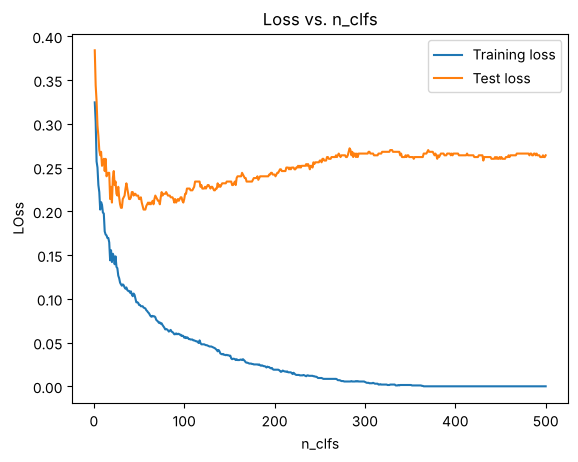
\includegraphics[width=0.48\textwidth]{../figs/fig3_gb_loss.png}\hfill
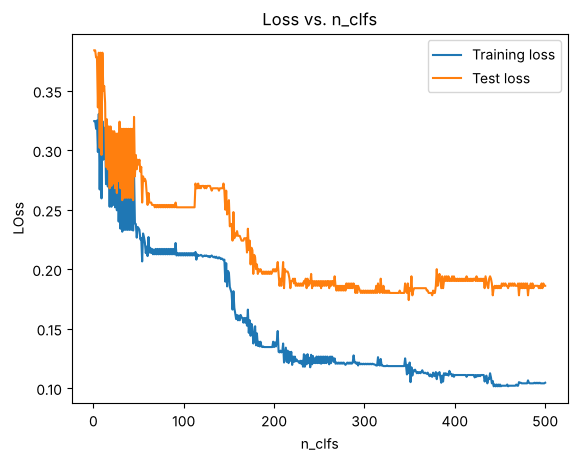
\includegraphics[width=0.48\textwidth]{../figs/fig3_ab_loss.png}
\end{center}
\emph{Smoothness.} Gradient boosting (left) is smooth: each regressor is fit to the residual, so every step makes a small change to the ensemble and the training loss falls almost monotonically.
AdaBoost (right) is jagged and step-like, with the loss going up on many iterations. The 0/1 loss is not what AdaBoost optimizes (it greedily reduces the exponential bound), and one new learner with a large coefficient can flip many points at once.

\emph{Final values.} Gradient boosting reaches training loss $0$ (after about 365 regressors) because it keeps fitting the residuals, noise included. Its test loss is best around $0.20$ (about 55 regressors) and then creeps up to $0.264$, a sign of overfitting.
AdaBoost levels off at training loss $\approx0.105$ and test loss $\approx 0.186$ and does not overfit in this range. Later learners face weights concentrated on the noisy overlap region, where they do barely better than chance ($\epsilon_t\approx0.497$, $\alpha_t\approx0.006$),
so they hardly change the ensemble.
\end{solution}

\begin{problem}[2]
    Compare the final loss values of the two models. Which performed better on the classification dataset?
\end{problem}
\begin{solution}
\upshape
Gradient boosting has the lower training loss ($0$ vs.\ $0.105$), but AdaBoost has the lower test loss ($0.186$ vs.\ $0.264$). Since test loss measures generalization, AdaBoost performed better on this classification dataset.
\end{solution}

\begin{problem}[2]
    For AdaBoost, where are the dataset weights the largest, and where are they the smallest?
\end{problem}
\begin{hint}
    Watch how the dataset weights change across time in the animation.
\end{hint}
\begin{solution}
\upshape
\begin{center}
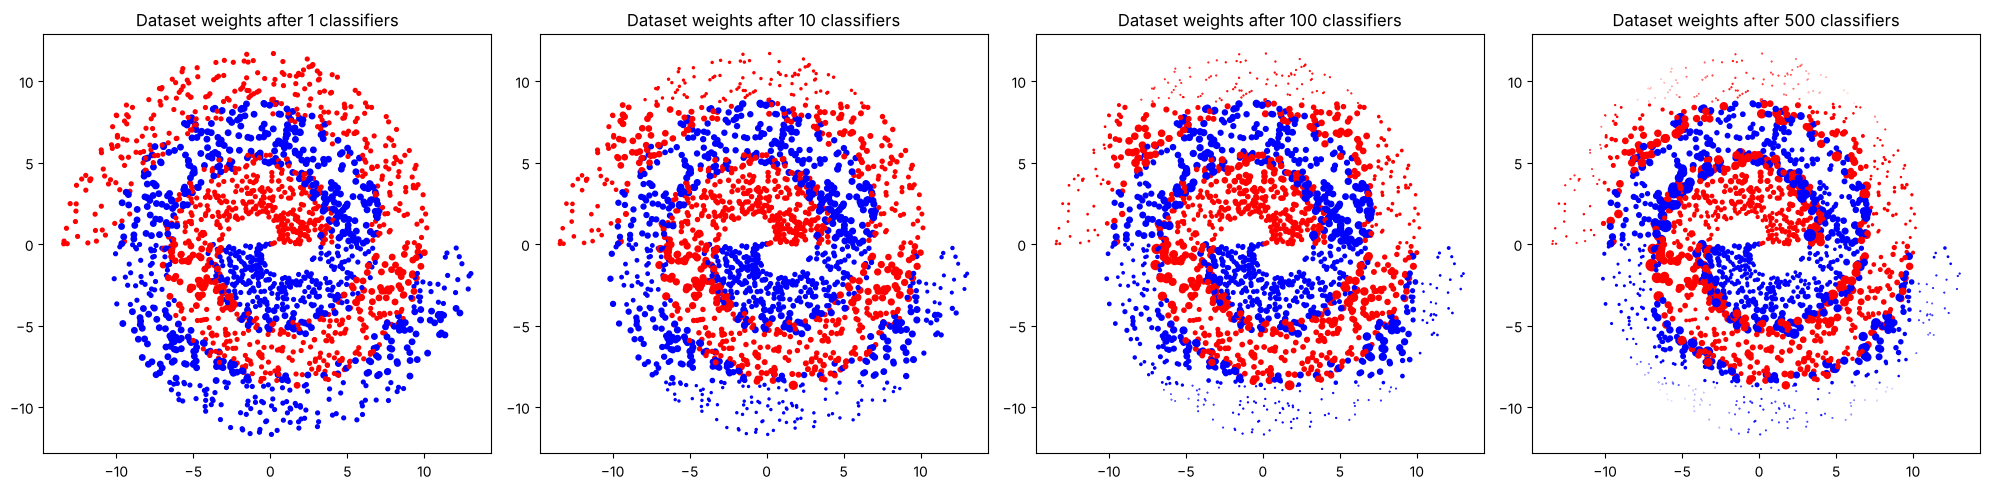
\includegraphics[width=\textwidth]{../figs/fig3_ab_weights.png}
\end{center}
The weights are largest for points in the band where the two spirals overlap, i.e.\ near the decision boundary and among the noisy points, which are repeatedly misclassified.
For example, the final weight of the training points the ensemble gets wrong averages $1.5\times10^{-3}$, vs.\ $3.8\times10^{-4}$ for points it gets right.
The weights are smallest for points far from the boundary, such as the outer ends of the spiral arms (radius above 12), which are classified correctly from the first few rounds and keep being down-weighted.
Their weights shrink exponentially, down to about $10^{-7}$.
\end{solution}

\end{document}
